% !TeX root = main.tex
\section{2.3 - Analyzing Lucas-Kanade Method}

\subsection{Local structure-tensor rank}

\paragraph*{Question}
\begin{displayquote}
    Why is optical flow only valid in the regions where local structure-tensor $A^\top A$ has a rank 2? What role does the threshold $\tau$ play here?
\end{displayquote}

The equation of Optical Flow is given by

\begin{equation*}
    \mathbf{h} = \begin{bmatrix} h_x & h_y \end{bmatrix} = \left [ \sum_{\mathbf{x} \in R} \begin{pmatrix}
        \frac{\partial F}{\partial x} & \frac{\partial F}{\partial y}
        \end{pmatrix} \left( G(\mathbf{x}) - F(\mathbf{x}) \right ) \right ] {\underbrace{\begin{bmatrix}
        \sum_{\mathbf{x} \in R} \left ( \frac{\partial F}{\partial x} \right )^2 &
        \sum_{\mathbf{x} \in R} \left ( \frac{\partial F}{\partial x} \right ) \left ( \frac{\partial F}{\partial y} \right ) \\
        \sum_{\mathbf{x} \in R} \left ( \frac{\partial F}{\partial x} \right ) \left ( \frac{\partial F}{\partial y} \right ) &
        \sum_{\mathbf{x} \in R} \left ( \frac{\partial F}{\partial x} \right )^2
        \end{bmatrix}}_{A^\top A}}^{-1}
\end{equation*}

The structure tensor $A^\top A$ should be \emph{invertible} to find the optical flow $\mathbf{h}$. This happens only when the matrix $A^\top A$ is \emph{well-conditioned}; otherwise, the inverse will be unstable. Using the rank of $A^\top A$ is a good proxy. The matrix will be invertible when $A^\top A$ has a rank of 2.

The threshold $\tau$ allows eliminating cases where the matrix $A^\top A$ is poorly conditioned. That is, the value of $\sfrac{\sigma_1}{\sigma_2}$ is used to determine the stability of inverse ($\sigma_1$ is the greater eigenvalue and $\sigma_2$ the smaller - this result should be close to 1). Using a threshold (eliminating the values where the smaller eigenvalue is less than a small value) allows eliminating unstable optical flow points.

\subsection{Modifications}

\paragraph*{Question}
\begin{displayquote}
    In the experiments, did you use any modifications and/or thresholds? Does this algorithm work well for these test images? If not, why?
\end{displayquote}

Several test images were used in the \texttt{Assignment02.ipynb} file. One modification was the implementation of a quick Lukas-Kanade in a grid.

\begin{figure}[h]
    \centering
    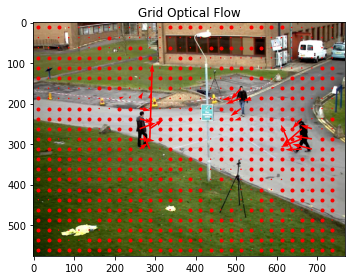
\includegraphics[width=0.6\textwidth]{grid_opt_flow.png}
    \caption{Lukas-Kanade in a grid}
    A test image which wasn't in the given data.
\end{figure}

In some cases, the algorithm works well (the best result is shown in the notebook). However, in some cases, the algorithm fails to find good flow vectors. This is true in cases where there isn't a large amount of consistency in the environment or when there is an affine transform.

The LK method assumes that the error is gaussian. It can be extended for affine settings.

\subsection{Window Size}

\paragraph*{Question}
\begin{displayquote}
    Try experimenting with different window sizes. What are the trade-offs associated with using a small versus a large window size? Can you explain what's happening?
\end{displayquote}

A smaller window size gives more accurate results but takes longer to compute. A tiny window size might give a lot of false matches (since there could be more regions that closely correspond to a small patch).

If the window size is too large, then the point will not move like its neighbors (because matching won't find an exact match). Things might enter or leave the large window. There could be occlusions. There could even be cases where shadows are differently formed.

\subsection{Failure points of LK method}

\paragraph*{Question}
\begin{displayquote}
    There are locations in an image where Lucas-Kanade optical flow will fail, regardless of the choice of window size and sigma for Gaussian smoothing. Describe two such situations. You are not required to demonstrate them.
\end{displayquote}

The following situations could be where the Lukas Kanade tracker fails

\begin{itemize}
    \item \textbf{Occlusions and shadows}: If corners get occluded, we will not be able to find the similar patch in the neighborhood. If there is illumination such that the shadows move quickly, it could give some false optical flow.
    \item \textbf{In-plane rotations}: If there is an in-plane rotation, pixels away from the center of rotation could have high optical flow. If the rotation speed is very high, then the pixels could have high shift. In such cases, the slow motion assumption could be violated. Optical flow in these cases will fail.
    \item \textbf{Lack of features}: If no features can be detected, then optical flow cannot be found. Changing any parameter will not fix this. Consider a planar surface with no illumination gradient, moving in a scene. No optical flow can be found on the surface.
\end{itemize}

\subsection{HSV Visualization}

\paragraph*{Question}
\begin{displayquote}
    Did you observe that the ground truth visualizations are in HSV colour space? Try to reason it.
\end{displayquote}

HSV properly separates color information (hue or chroma) and illumination (value or luma). By converting the optical flow vectors to polar coordinates, we can map the angle to color (in 0 to 180 range) and magnitude to the illumination.

This way, pixels that have high optical flow will have high illumination, whereas pixels with low motion will have low illumination (near black). The color of the pixel will give a sense of direction.
